\documentclass[c,10pt,pdftex]{beamer}
\usepackage[T1]{fontenc}
\usepackage[utf8]{inputenc}
\usepackage[english]{babel}

\hypersetup{
  colorlinks=true,
  urlcolor=blue
}

% \usepackage{ucs} % for utf8x

\usepackage{graphicx}

% the following packages are for pseudocode
\usepackage{algorithm2e}
\usepackage{algorithmic}
\usepackage{float}

\usepackage[autostyle, italian=guillemets]{csquotes}
\usepackage[backend=biber]{biblatex}
\addbibresource{seminar.bib}
\usetheme{tb}


\title{Transport networks and road safety}

% Nom de l'auteur
\author{Andrea Gilardi \inst{1} \and Robin Lovelace \inst{2}}
\institute{\inst{1} University of Milan - Bicocca \and \inst{2} University of Leeds - ITS}

\begin{document}

\inserttitlepage

\begin{frame}
\frametitle{Who am I}
\vspace{-0.75cm}
\begin{itemize}
	\setlength\itemsep{1em}
	\item I'm Andrea Gilardi, a Ph.D. student in Statistics at the University of Milan - Bicocca. 
	\item My main research interests lie in the field of spatial and spatiotemporal statistics, with a particular focus on point pattern events on a linear network. I really love coding in R. 
	
	\item Now I'm in Leeds (I will leave next week unfortunately) working with Robin Lovelace on a review of existing packages for spatial network analysis in R (like \texttt{stplanr}) improving my knowledge on several spatial topics and applying statistical methods to road safety research
\end{itemize}
\end{frame}

\begin{frame}
\frametitle{Overview of the seminar}
\begin{itemize}
	\item In the first part of the seminar I will present you the basics idea behind the graph representation of a street network. We will see three common pitfalls on OpenStreetMap highway data and how to solve them. 
	
	\item In the second part I will show you some methods that we used to explore the distribution of car crashes occurred in 2018 on the street network of the Isle of Wight.
	
	\item In the third and last part of this seminar I will present you an Empirical Bayes methodology for the estimation of a road risk index on a street network.  
\end{itemize}
\end{frame}

\begin{frame}
\frametitle{A few definitions}
\vspace{-0.75cm}
\begin{itemize}
	\setlength\itemsep{1em}
	\item Informally, a Point Process is a random mechanism whose outcomes are Point Patterns, i.e. a (finite) sequence of points in the space. 
	
	\item Classical examples of point processes are: tree locations in a forest (the classic swedish pines data), animal nesting sites, ambulance interventions or, as  in this seminar, \alert{car crashes}. 
	
	\item We will use these data to formalize the first steps we took towards the definition of a precise model that can be used to locate the most dangerous locations for car crashes (i.e. the black spots). 
\end{itemize}
\end{frame}

\begin{frame}
\frametitle{Car crashes data}
\vspace{-0.75cm}
\begin{itemize}
	\setlength\itemsep{1em}
	\item In the following part of this seminar, we will analyze the data of all car crashes that occurred in the \alert{Isle of Wight (UK) during 2018}. 
	
	\item We downloaded the data using the \texttt{stats19} package, which is a tool to help download, process and analyse the UK road collision data collected using the 'STATS19' form. 
	
	\item These data are really rich and they include several additional information (like the severity of the crash, the weather, the light condition and several other markers) but, for the moment, we will focus only on the location of the events. 
\end{itemize}
\end{frame}

\begin{frame}
\frametitle{Car crashes data (cont)}
\vspace{-0.25cm}
This is a graphical representation of the car crashes occurred in the Isle of Wight (UK) during 2018. There are some clear patterns in the data that we need to take into account.
\begin{figure}
	\centering
	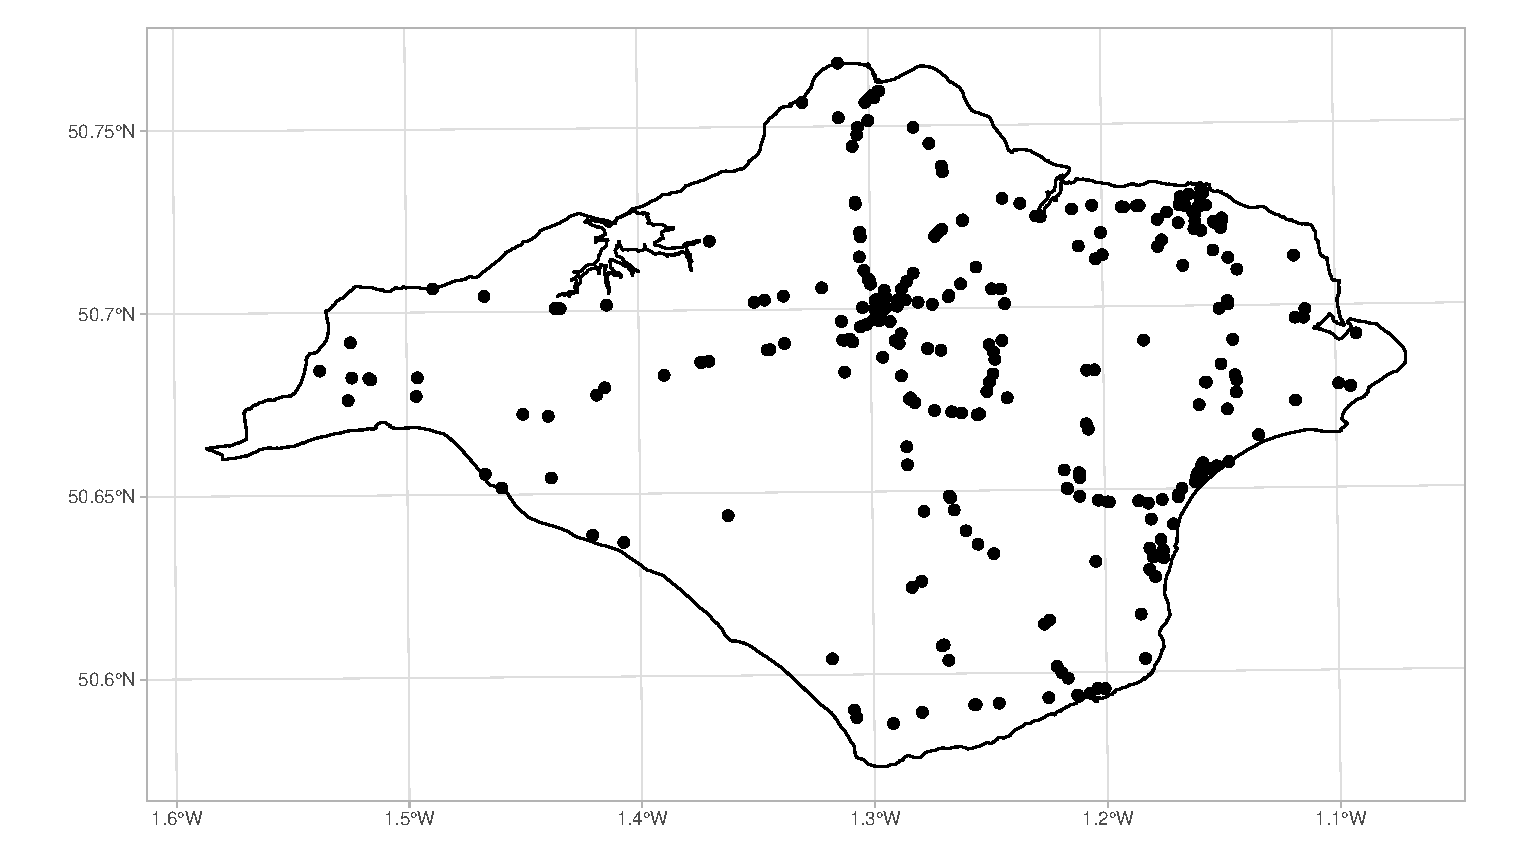
\includegraphics[width=\linewidth]{images/iow_crashes}
\end{figure}
\end{frame}

\begin{frame}
\frametitle{Point Processes on a Street Network}
\vspace{-0.25cm}
Car crashes represent a classical example of a \alert{point process occurring on a linear network}. The usual statistical techniques (such as the following quadratcount) are not valid. 
\vspace{-0.5cm}
\begin{figure}
	\centering
	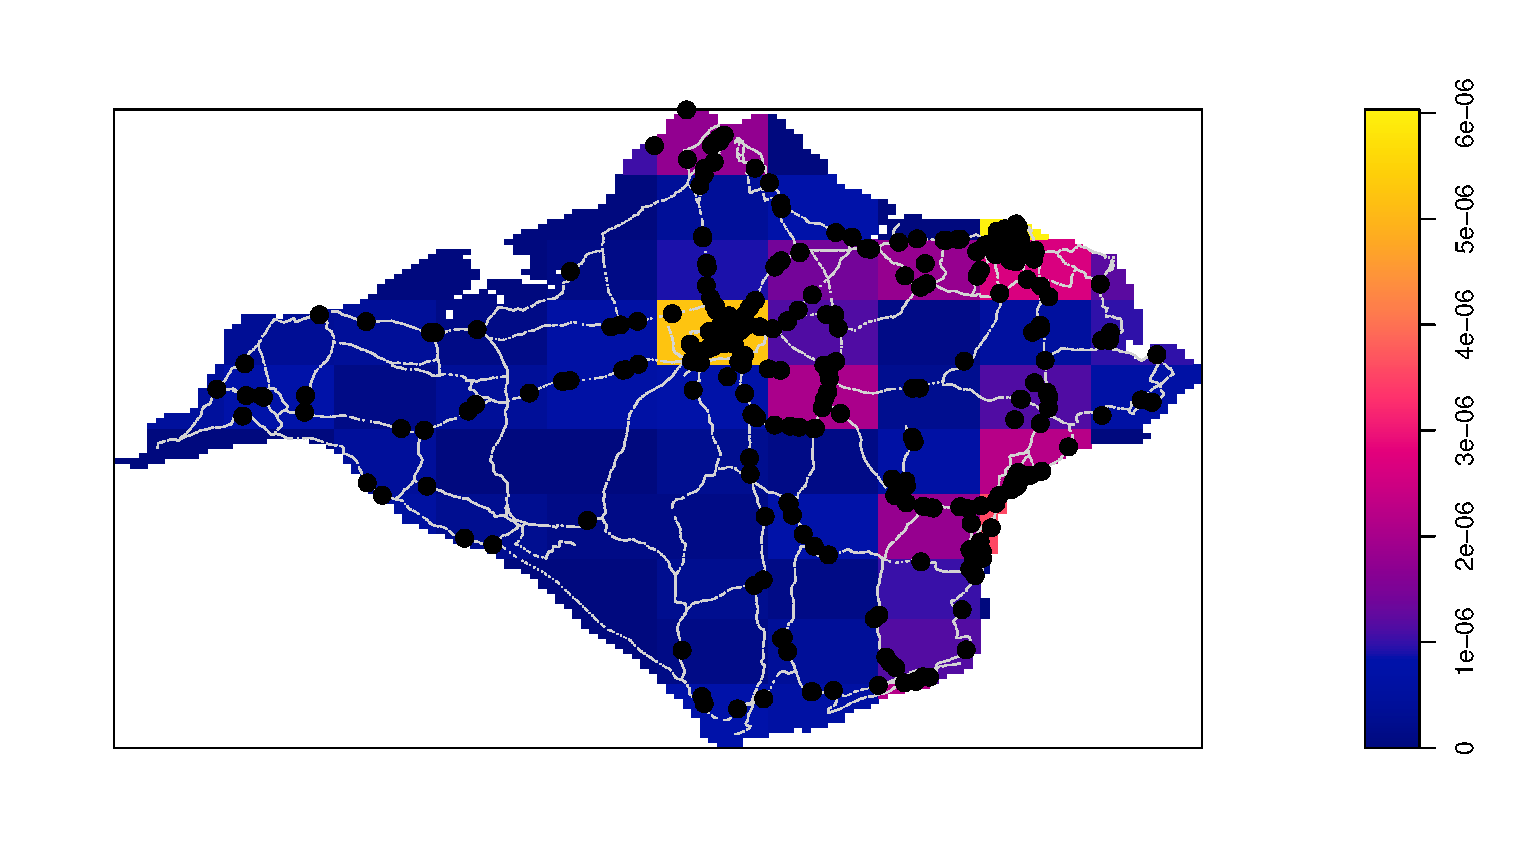
\includegraphics[width=\linewidth]{images/quadratcount2}
\end{figure}
\end{frame}

\begin{frame}
\frametitle{Street Networks}
\vspace{-0.75cm}
\begin{itemize}
  \setlength\itemsep{1em}
  \item The road network we use is built using \alert{OpenStreetMap} data. 
  \item OpenStreetMap is a project that aims at building a free and editable map of the World with an open-content license. 
  \item The basic components of OpenStreetMap data are called \textit{elements} and they consist of: 
  \begin{itemize}
    \setlength\itemsep{0.25em}
    \item \textit{nodes}: representing points on the earth surface; 
    \item \textit{ways}: which is an ordered list of nodes; 
    \item \textit{relations}: which is a list of nodes, ways and other relations. Each member has additional information that describe its relationship with the other elements. Roads, turn restrictions and administrative boundaries are usually described as relations.
  \end{itemize}
\end{itemize}
\end{frame}

\begin{frame}
\frametitle{Street Network in the Isle of Wight}
This is a graphical representation of the main roads in the Isle of Wight. 
\vspace{-0.75cm}
\begin{figure}
\centering
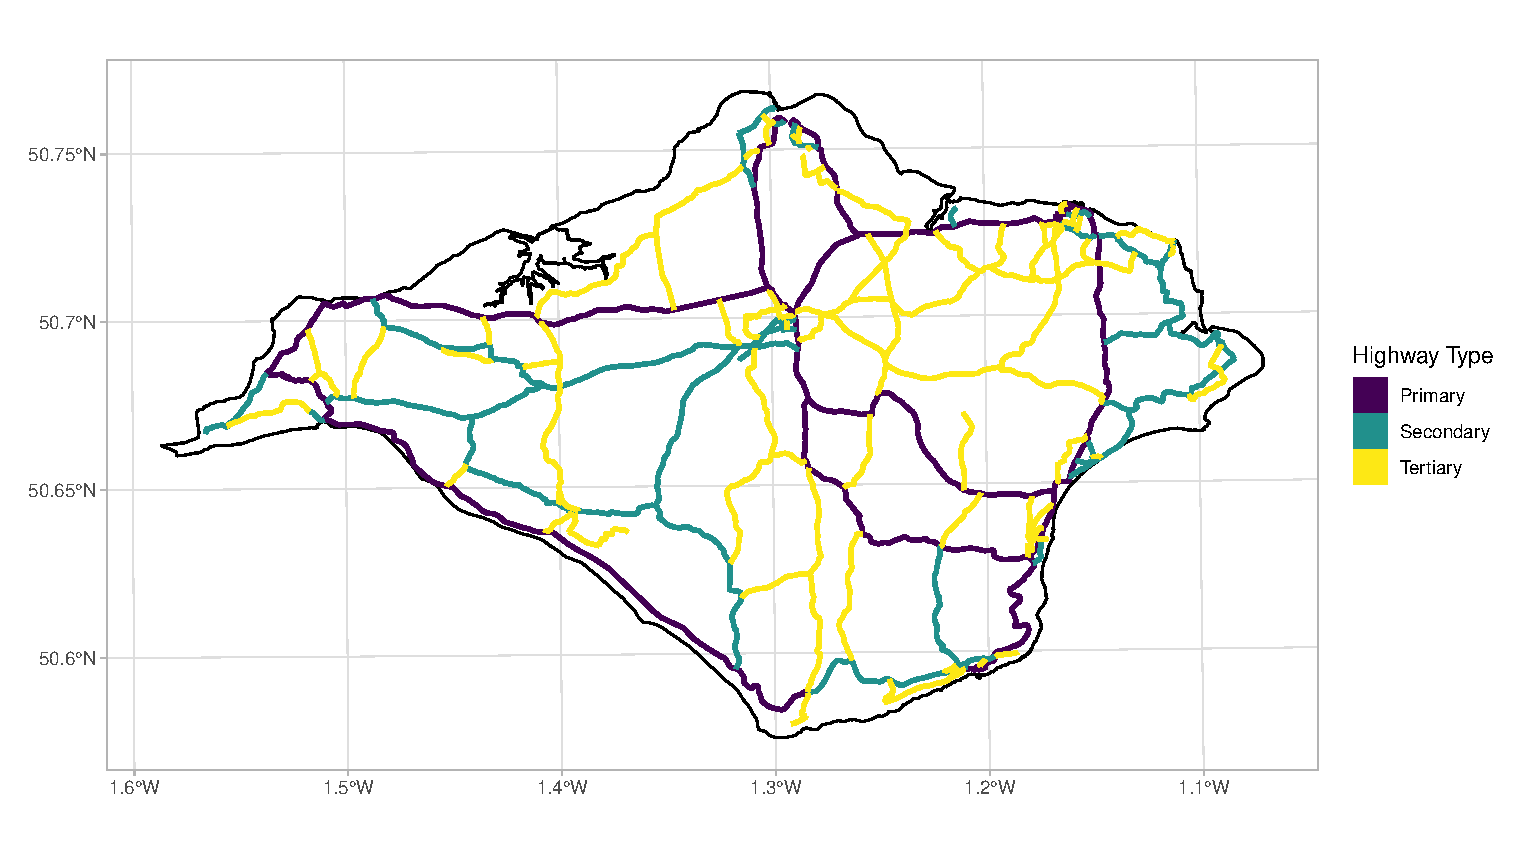
\includegraphics[width = 1.05\linewidth]{images/highway_type}
\end{figure}
\end{frame}

\begin{frame}
  \frametitle{Representing street networks as graphs}
  \vspace{-0.75cm}
  \begin{itemize}
    \setlength\itemsep{1em}
    \item Typically roads are represented purely as geographic objects, but they are also \alert{graphs}
    \item A few ways of representing spatial networks have been developed, including in the R package \texttt{stplanr}
    \item That is, roughly speaking, how Robin and I met
  \end{itemize}
  \begin{figure}
  	\centering
  	
\includegraphics[width = 1.05\linewidth]{images/stplanr-wide-screenshot}
  \end{figure}	
\end{frame}

% \begin{frame}
%   \frametitle{Getting road crash data with the stats19 package}
%   % suggestion: demonstrate code for getting stats19, say we taught it in London
% \end{frame}
% 
% \begin{frame}
%   \frametitle{Getting road network data}
%   % Mention that it's easier than ever to get OSM data, thanks to another package we developed?
% \end{frame}

\begin{frame}
  \frametitle{\texttt{stplanr} - networks}
  \vspace{-0.75cm}
  \begin{itemize}
    \setlength\itemsep{1em}
    \item Broadly speaking, let's say that a \alert{street network} is a graph whose nodes and edges are associated with geographical elements in the space. 
    \item In the \texttt{stplanr} representation of a street network, the edges are the ways that were download from OSM while the vertexes are the starting and ending node of each way. 
    \item This representation implies that two or more edges are \textit{connected} if and only if they share one or more boundary point. 
  \end{itemize}
\end{frame}

\begin{frame}
  \frametitle{Problems...}
  \vspace{-0.5cm}
  Theories and definitions are fine but obviously the data we face in the wild world is quite different. We will discuss three probems: \alert{roundabouts} (i.e. circular ways), \alert{overpasses} (i.e. intersecting ways that are not really connected due to a vertical grade of separation) and (some) \alert{street intersections}.  
  \begin{columns}
  	\begin{column}{0.5\linewidth}
  		\begin{figure}
  			\centering
  			\Large \textbf{Theory} \par \medskip
  			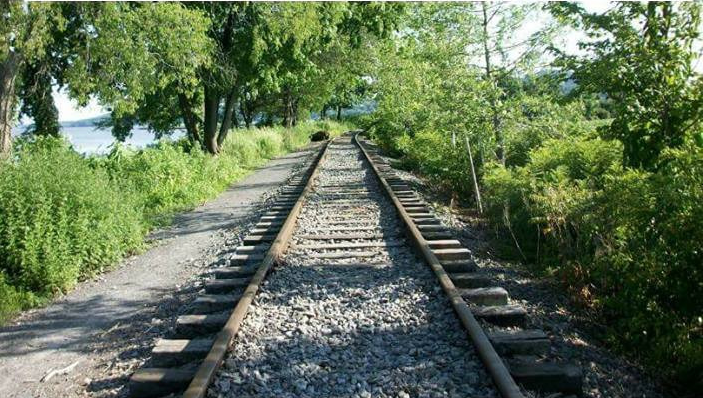
\includegraphics[width = \linewidth]{images/theory.png}
  		\end{figure}
  	\end{column}
  	\begin{column}{0.5\linewidth}
  		\begin{figure}
  			\centering
  			\Large \textbf{Real Data} \par \medskip
  			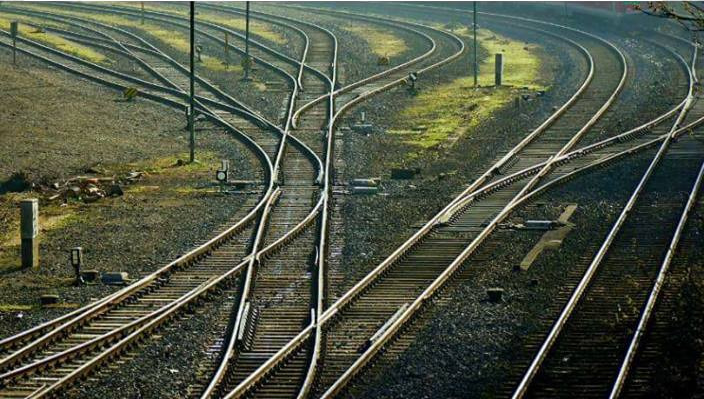
\includegraphics[width = \linewidth]{images/real_data.png}
  		\end{figure}
  	\end{column}
  \end{columns}
\end{frame}

\begin{frame}
  \frametitle{Roundabouts, i.e. circular ways}
  \vspace{-0.25cm}
  The street network on the left is unroutable by \texttt{stplanr}-definition since the roundabout is not connected to the other edges.  
  \vspace{-0.25cm}
  \begin{columns}
    \begin{column}{0.5\linewidth}
      \begin{figure}
      \centering
      \large \textbf{Before} \par \medskip
      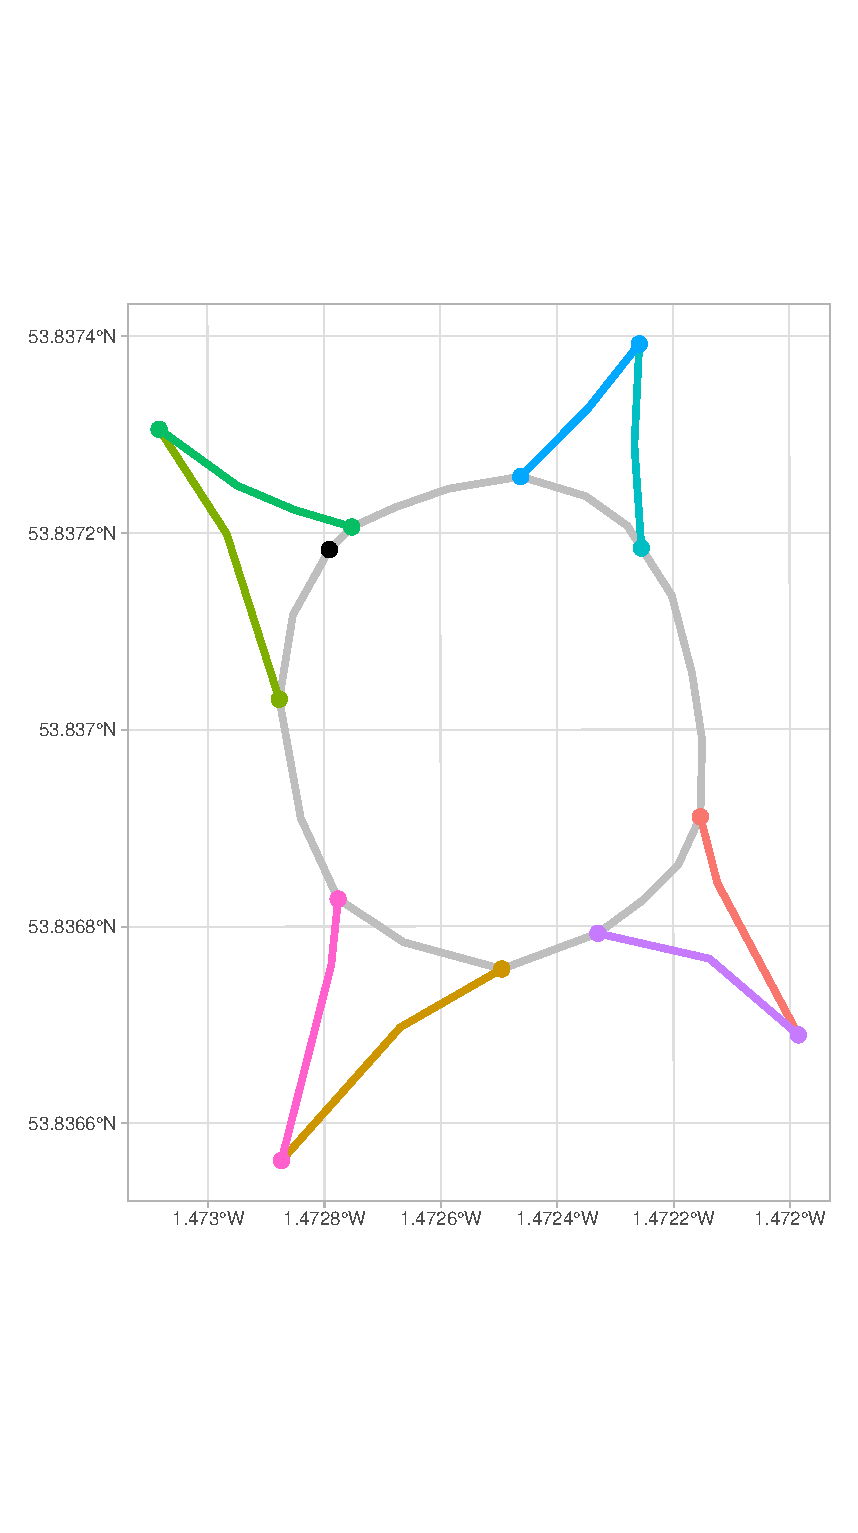
\includegraphics[width = 0.9\linewidth, trim = {0 0 0 4cm}, clip]{images/roundabout1}
      \end{figure}
    \end{column}
    \begin{column}{0.5\linewidth}
      \begin{figure}
      \centering
      \large \textbf{After} \par \medskip
      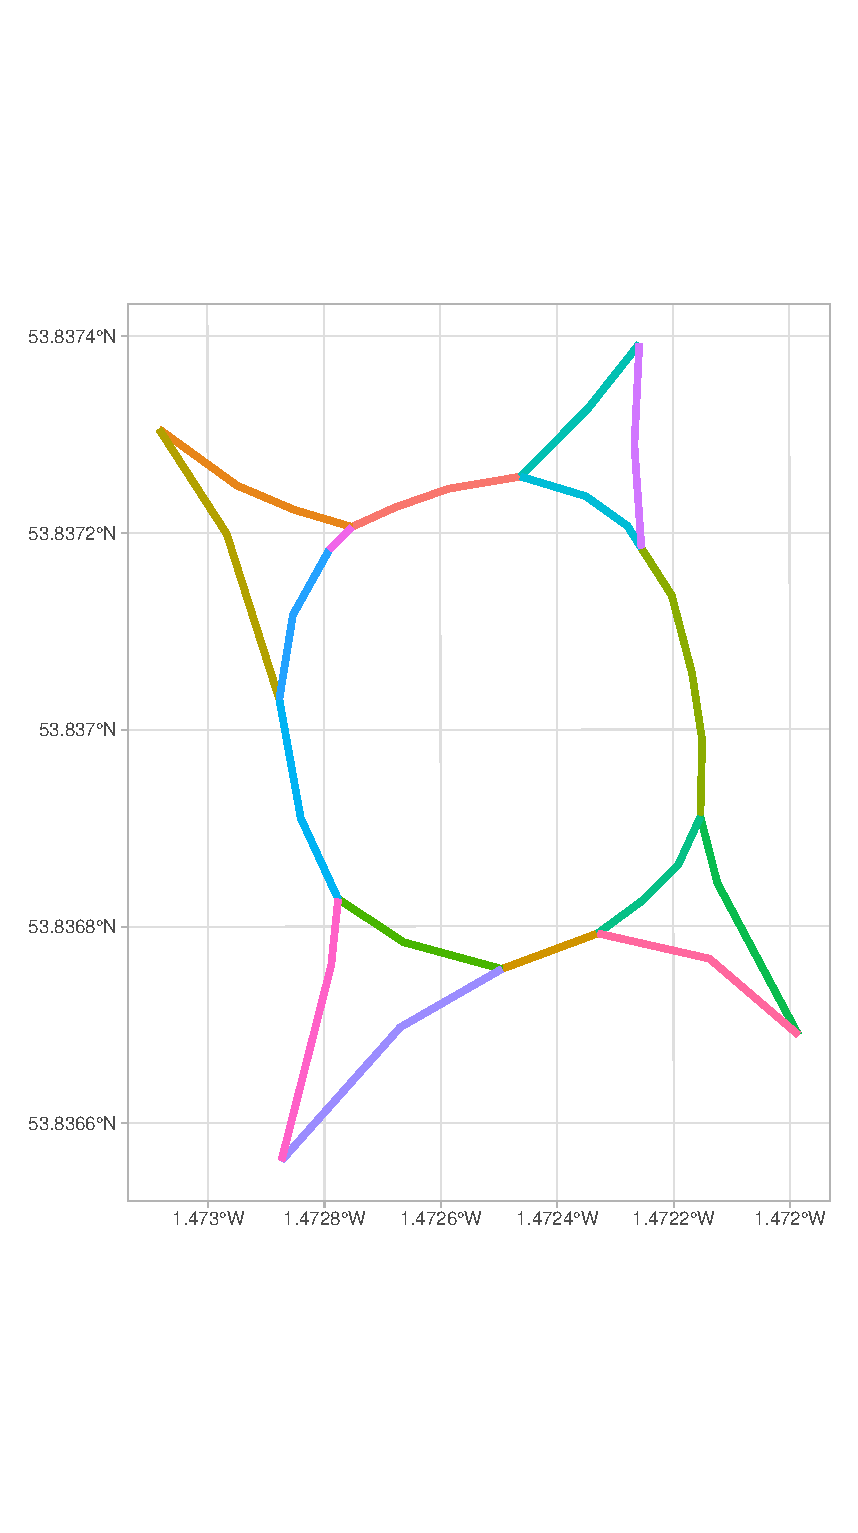
\includegraphics[width = 0.9\linewidth, trim = {0 0 0 4cm}, clip]{images/roundabout2}
      \end{figure}
    \end{column}
  \end{columns}
\end{frame}

\begin{frame}
\frametitle{Bridges, overpasses and underpasses}
\vspace{-0.75cm}
Even if we break up a street network we must be sure not to ruin overpasses and underpasses relations. 
\begin{columns}
	\begin{column}{0.5\linewidth}
		\begin{figure}
			\centering
			\large \textbf{Before} \par \medskip
			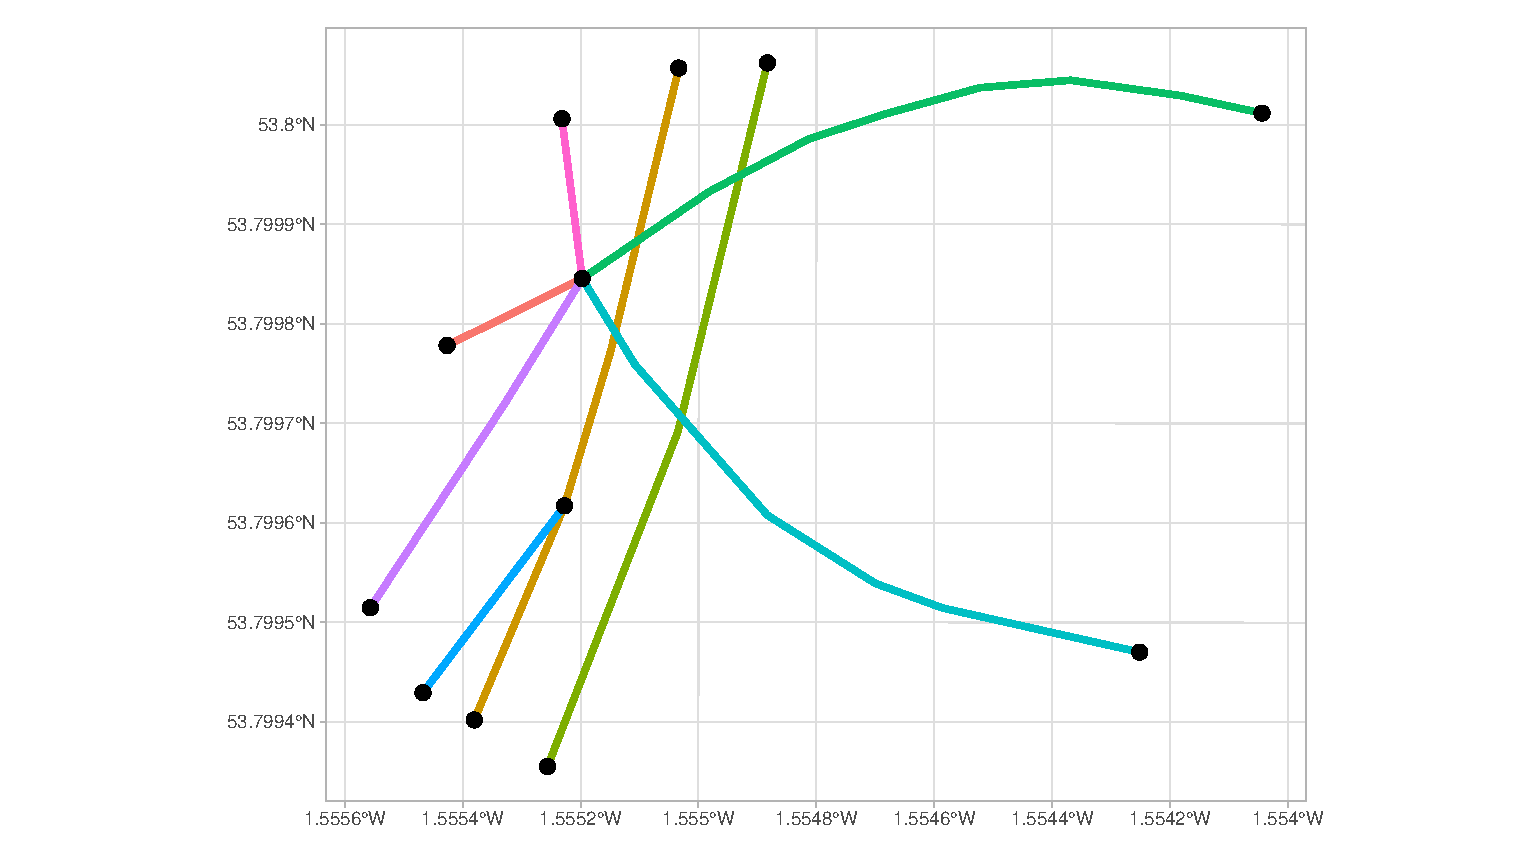
\includegraphics[width = \linewidth, trim = {4cm 0 3.75cm 0}, clip]{images/overpasses1}
		\end{figure}
	\end{column}
\begin{column}{0.5\linewidth}
	\begin{figure}
		\centering
		\large \textbf{After} \par \medskip
		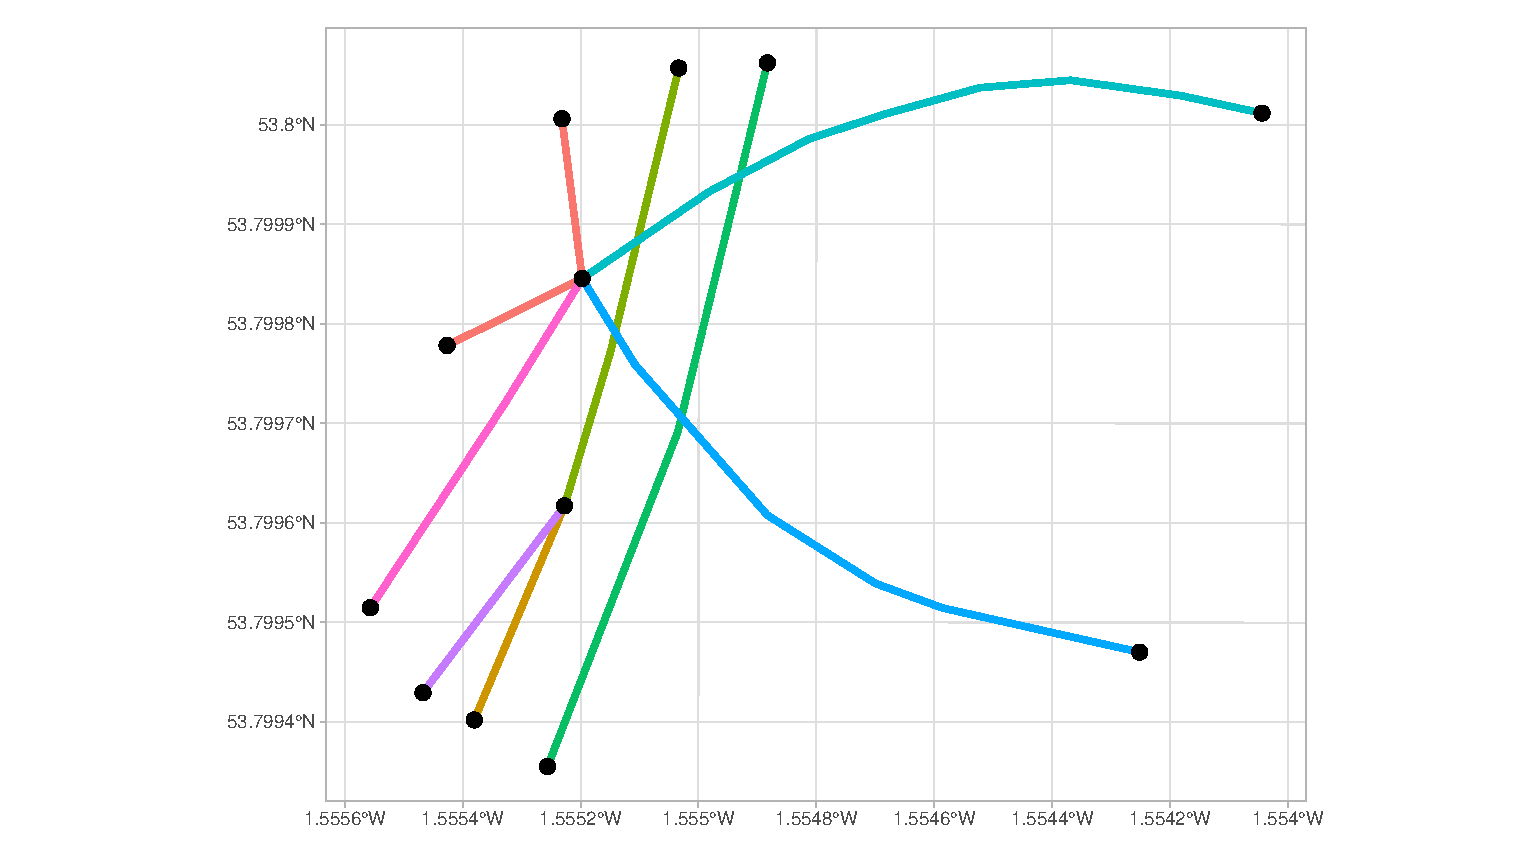
\includegraphics[width = \linewidth, trim = {4cm 0 3.75cm 0}, clip]{images/overpasses2}
	\end{figure}
\end{column}
\end{columns}
\end{frame}

\begin{frame}
\frametitle{Streets intersections}
\vspace{-0.75cm}
There are also some cases where two streets intersects and they don't share any vertex.
\begin{columns}
	\begin{column}{0.5\linewidth}
		\begin{figure}
			\centering
			\large \textbf{Before} \par \medskip
			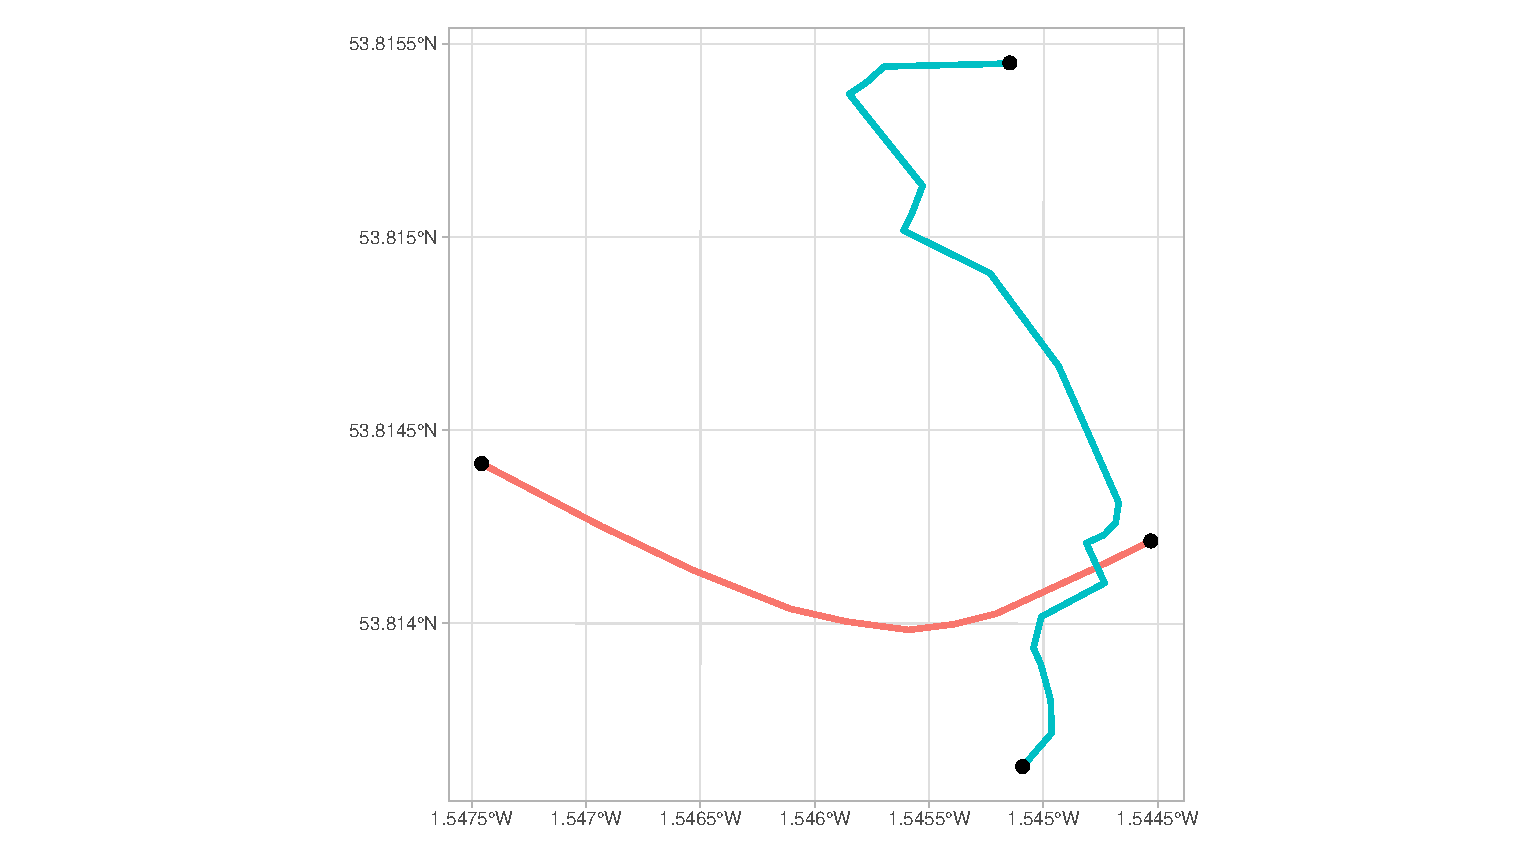
\includegraphics[width = \linewidth, trim = {5.5cm 0 4.5cm 0}, clip]{images/intersections1}
		\end{figure}
	\end{column}
\begin{column}{0.5\linewidth}
	\begin{figure}
		\centering
		\large \textbf{After} \par \medskip
		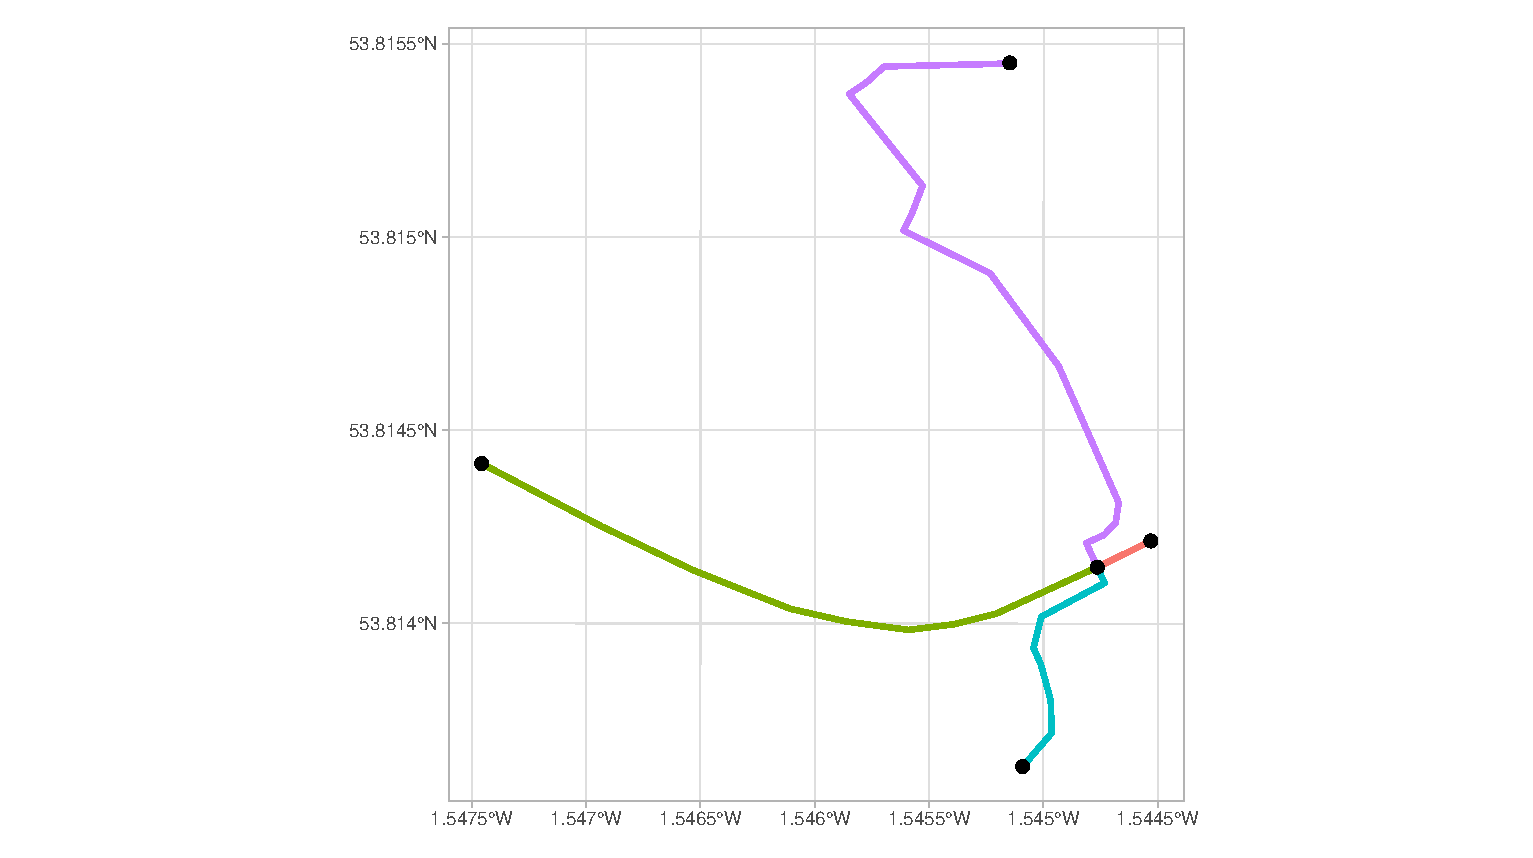
\includegraphics[width = \linewidth, trim = {5.5cm 0 4.5cm 0}, clip]{images/intersections2}
	\end{figure}
\end{column}
\end{columns}
\end{frame}

\begin{frame}
\frametitle{Fixing the street networks}
\vspace{-0.25cm}
We developed a new function (called \texttt{rnet\_breakup\_vertices} and stored in \texttt{stplanr} package) to fix all these problems. This is the result. 
\begin{figure}
	\centering
	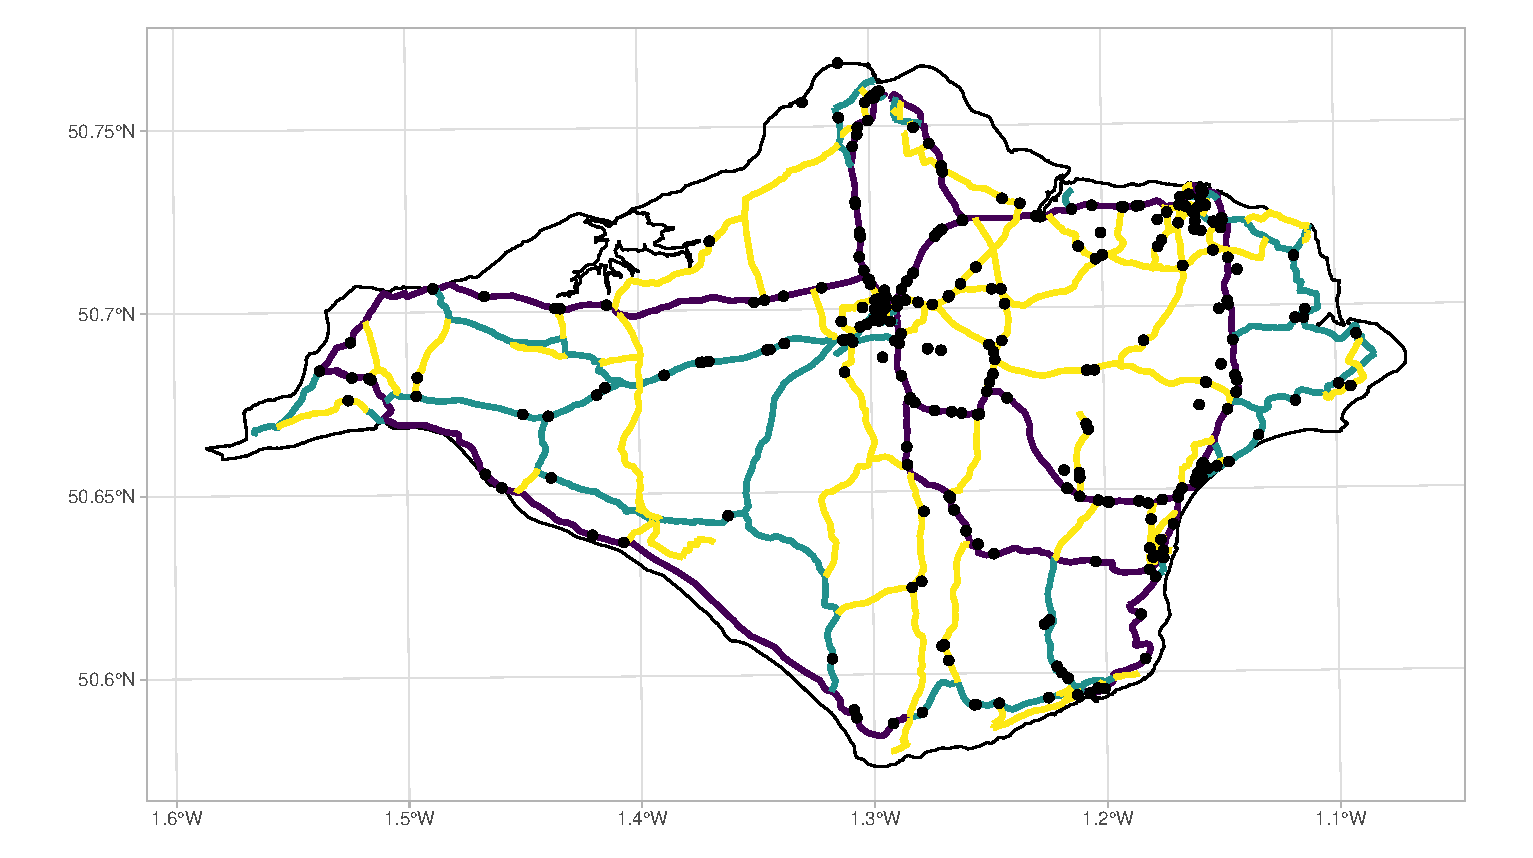
\includegraphics[width=\linewidth]{images/breaking_network}
\end{figure}
\end{frame}

\begin{frame}
\frametitle{Counting crashes on street networks}
\vspace{-0.75cm}
\begin{itemize}
	\setlength\itemsep{1em}
	\item Following the same ideas behind the quadratcounts procedure applied on the plane, we want to \alert{count the number of car crashes occurring on each edge of the street network}. 
	\item R can only represent exactly integers numbers and fractions whose denominator is a power of two \href{https://cran.r-project.org/doc/FAQ/R-FAQ.html\#Why-doesn_0027t-R-think-these-numbers-are-equal_003f}{(source)}, so none of the car crashes (whose coordinates are represented as double numbers with a 53 binary digits accuracy) lie exactly on the street network.
	\item For that reason we wrote a few R function to match each car crash with the nearest edge on the network and count the occurrences.
\end{itemize}
\end{frame}

\begin{frame}
\frametitle{The first road risk measure}
\vspace{-0.25cm}
This is the result. You should note that we excluded all car crashes that were farther than 100m from the nearest network edge (33  crashes). 
\begin{figure}
	\centering
	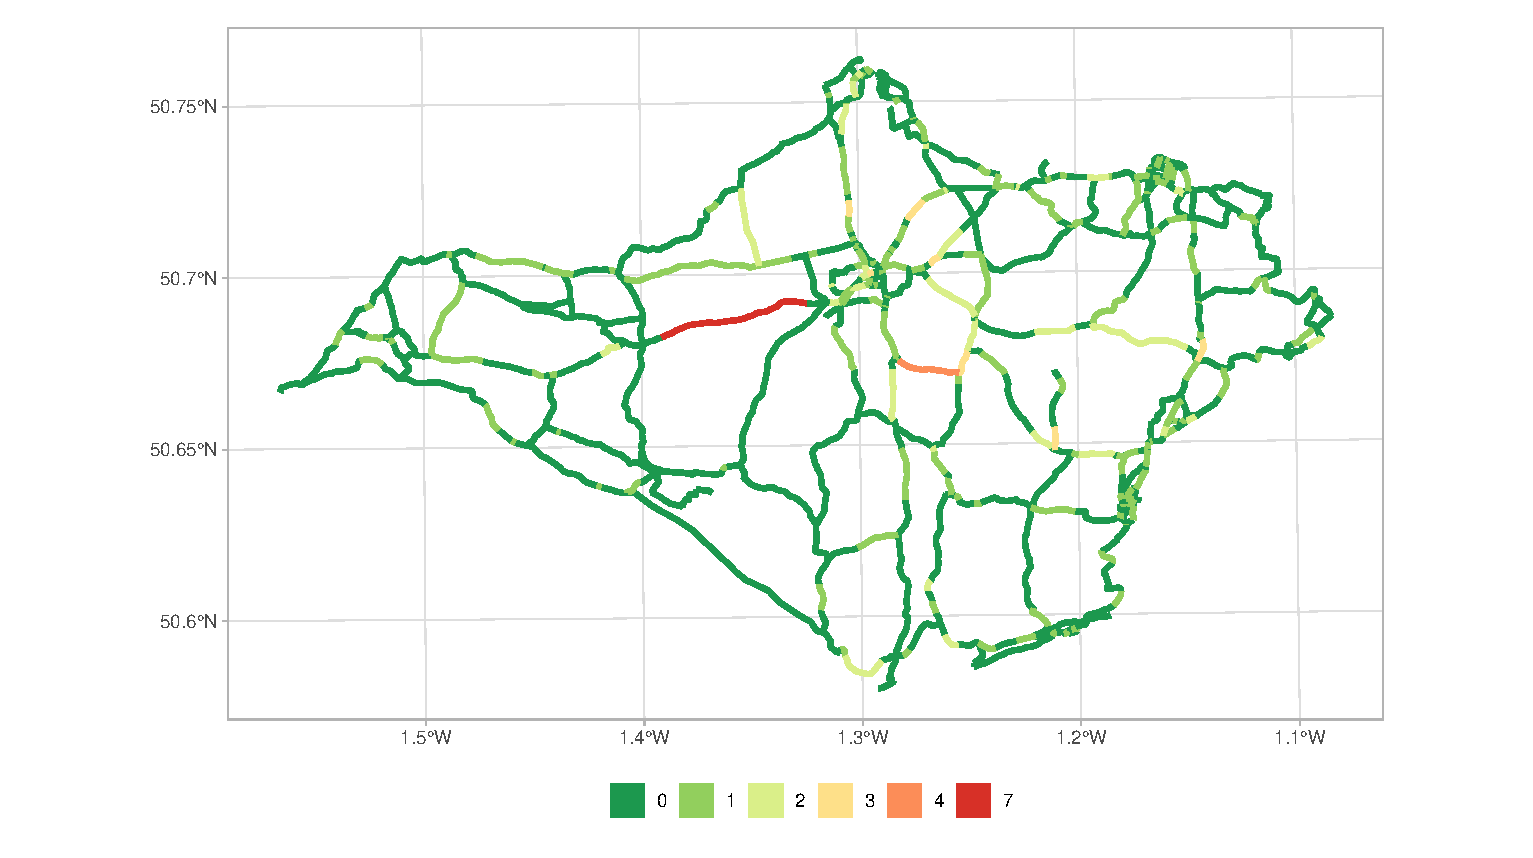
\includegraphics[width=\linewidth]{images/count_on_nearest_street}
\end{figure}
\end{frame}

\begin{frame}
\frametitle{Problems with the raw counts measure}
\begin{itemize}
	\setlength\itemsep{1em}
	\item There are some clear problems with the previous risk measure and, the most important one, is that we are comparing ways with very different length (i.e. different \textit{exposure}). 
	\item There are two possible solutions: 1) rebuild the network cutting and pasting ways in such a way that they all have approximately the same length; 2) \alert{estimate the number of car crashes per meter}. 
	\item For the moment we have to deal with the second solution since the other one is much more difficult to implement. 
\end{itemize}
\end{frame}

\begin{frame}
\frametitle{Car crashes per meter}
\vspace{-0.25cm}
This is the result and, then again, there are some obvious problems: there are a few car crashes occurring in very small road segments that artificially inflate this risk index.  
\begin{figure}
	\centering
	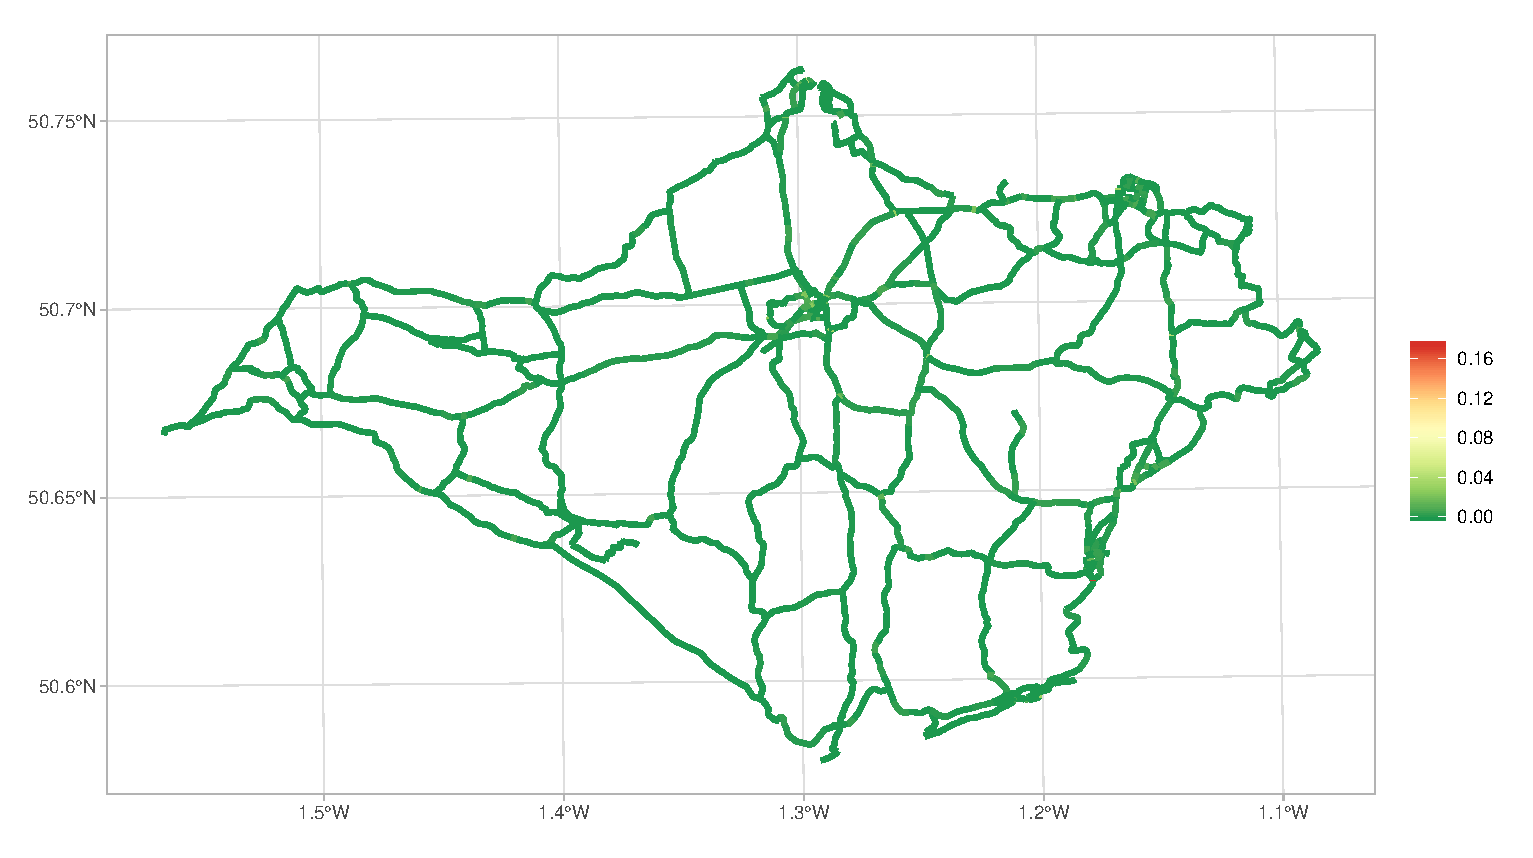
\includegraphics[width=\linewidth]{images/car_crashes_per_meter}
\end{figure}
\end{frame}

\begin{frame}
\frametitle{Local smoothing on a linear network}
\vspace{-0.75cm}
\begin{itemize}
	\setlength\itemsep{1em}
	\item Let $n$ be the number of (non overlapping) edges in the street network, $x_i, \ i = 1,\dots,n$ the number of car crashes occurring in each edge and $l_i, \ i = 1\dots n$ the length of each way. The ratio 
	\[
	y_i = \frac{x_i}{l_i}, \ i = 1, \dots, n
	\] 
	represent the number of car crashes per meter. 
	
	\item Let $\delta_{i, p}$ represent the set of all neighbours of each street $i$ up to order $p$. If $p = 0$ then $\delta_{i, p}$ includes only the $i$-th street segment; if $p = 1$ then $\delta_{i, 1}$ includes the street segment $i$ and its neighbours\footnote{In the \texttt{stplanr} representation of street networks, two ways are neighbours if they share one boundary point}; if $p = 2$ then $\delta_{i,2}$ includes the street segment, its neighbours and the neighbours of its neighbours and so on\dots
\end{itemize}
\end{frame}

\begin{frame}
\frametitle{Local smoothing on a linear network}
\vspace{-0.5cm}
\begin{itemize}
	\setlength\itemsep{1em}
	\item Now we can perform a \alert{local smoothing of $y_i$} as
	\[
	\tilde{y}_i = \frac{1}{m_i}\sum_{j \in \delta_{i, p}} y_{j} 
	\]
	where $m_i$ represent the number of elements included in $\delta_{i, p}$. 
	
	\item The value of $p$ is an input for the procedure and represent the degree of the smoothing: small values represent a local smoothing while higher values create a "global" smoothing. For example if we take $p = n$ then every segment is linked with the same value, i.e. $\tilde{y} = \frac{1}{n}\sum_{i=1}^{n}y_{i} \ \forall i = 1, \dots, n$. 
	
	\item The procedure was coded using the \texttt{igraph} package.
\end{itemize}
\end{frame}

\begin{frame}
\frametitle{Smoothing on a linear network}
\vspace{-0.25cm}
This is the result with $p = 6$ and now it's possible to extract some information from the plot. 
\begin{figure}
	\centering
	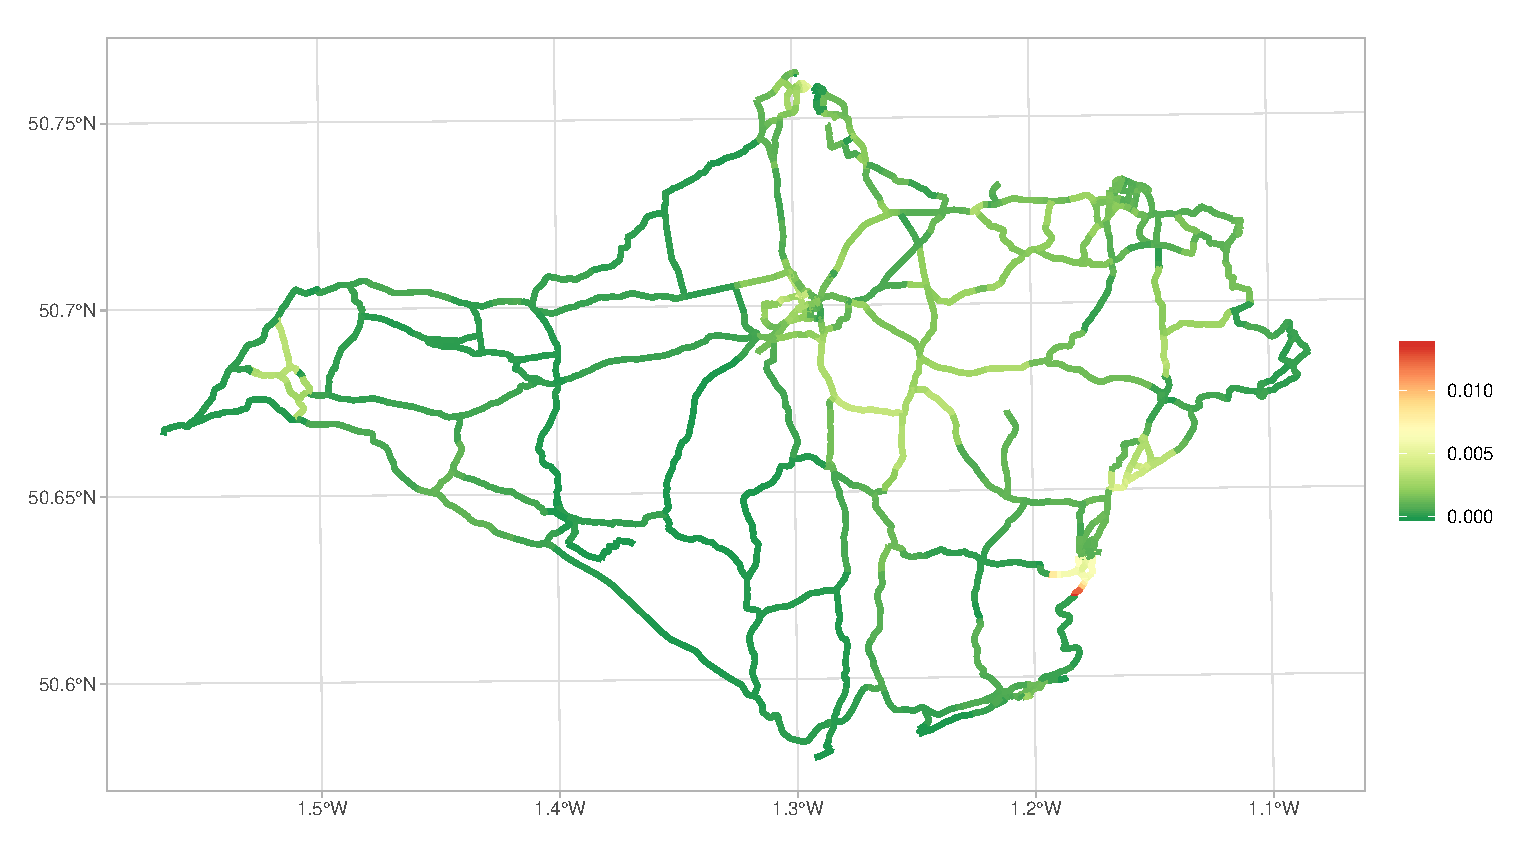
\includegraphics[width=\linewidth]{images/car_crashes_per_meter_smooth6}
\end{figure}
\end{frame}

\begin{frame}
\frametitle{Why network cleaning is important?}
\vspace{-0.25cm}
This is the same procedure applied to the street network without the cleaning and with $p = n$. It's clear that there is something wrong.
\begin{figure}
	\centering
	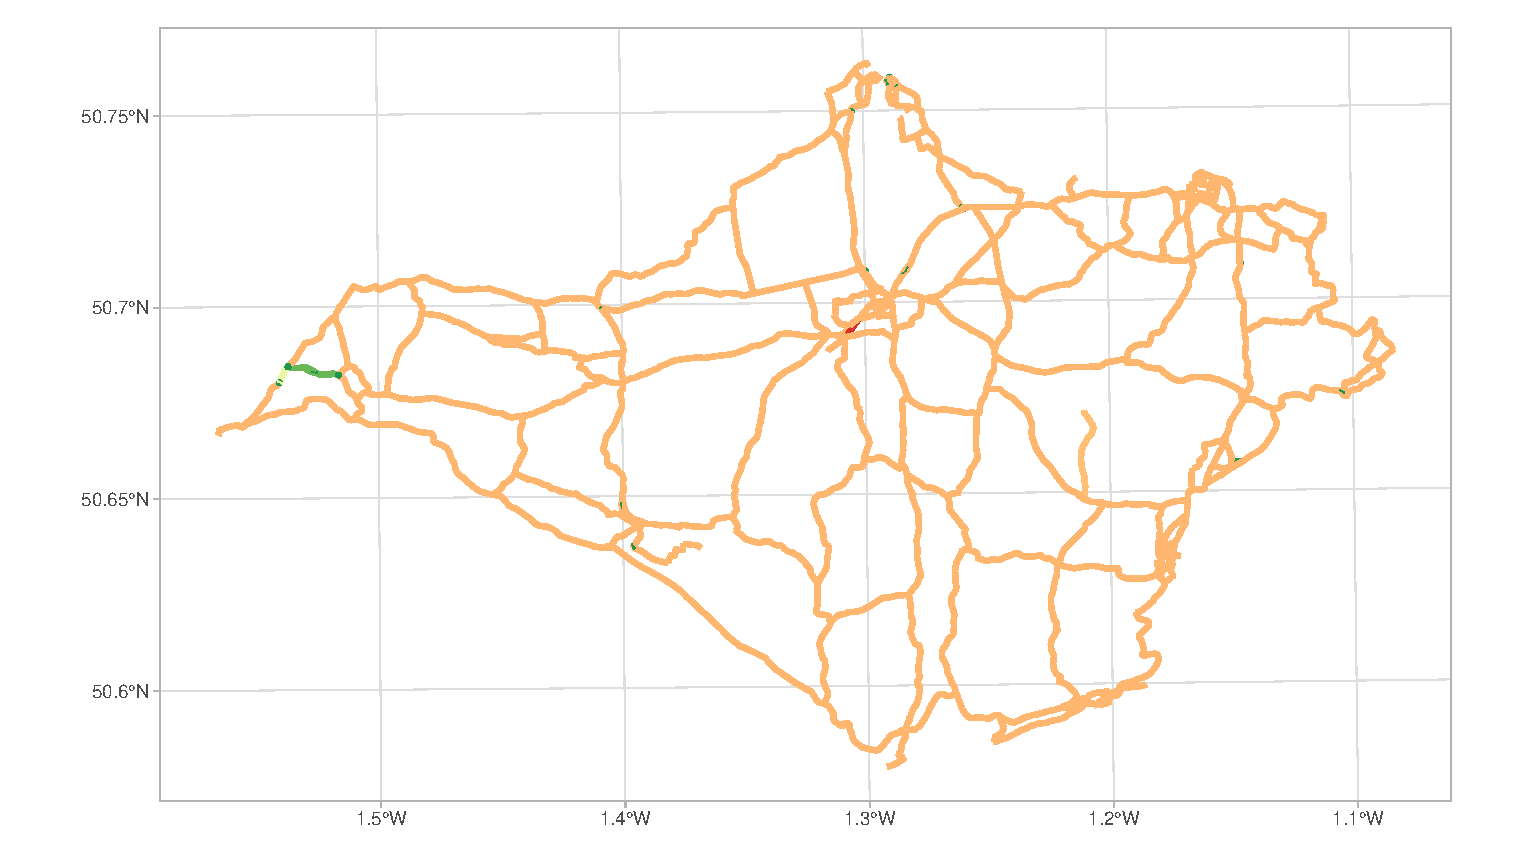
\includegraphics[width=\linewidth]{images/importance_of_network_cleaning}
\end{figure}
\end{frame}

\begin{frame}
\frametitle{Drawbacks}
\vspace{-0.75cm}
\begin{itemize}
	\setlength\itemsep{1em}
	\item Nevertheless, even if we work with a proper and clean network, the smoothing formula has several drawbacks since it is nothing more than an exploratory data analysis (EDA) procedure. 
	
	\item We did not define any precise statistical model which implies that we can't quantify any uncertainty measure on the risk indexes. Moreover, inference and testing procedures are not clearly defined. 
	
	\item In the last part of this seminar I'm going to present a statistical approach for the estimation of risk index on a street network which is based on \alert{Emprical Bayes Estimators}. 	
\end{itemize}
\end{frame}

\begin{frame}
\frametitle{Setting up the terminology}
\vspace{-0.75cm}
\begin{itemize}
	\setlength\itemsep{1em}
	\item  Let $n$ be the number of (non overlapping) edges in the street network and $x_i$ be the number of car crashes occurring in each edge. We assume that
	\[
	x_i \sim \alert{\text{Poisson}}(l_i\theta_i)
	\] 	
	where $l_i$ represents the \alert{exposure} on each segment and $\theta_i$ is the \alert{risk measure of the $i$th street segment}. 
	\item There are several possible ways to measure the exposure of each segment and, for the moment, we are going to assume that $l_i$ represents the \alert{length} of the $i$th segment. 
\end{itemize}
\end{frame}

\begin{frame}
\frametitle{Setting up the terminology (cont)}
\vspace{-0.75cm}
\begin{itemize}
	\setlength\itemsep{1em}
	\item We can now define 
	\[
	y_{i} = \frac{x_i}{l_i}
	\]  
	which is just the \alert{ratio between the number of car crashes and the length of the edge} and, under the previous assumptions, represent the maximum likelihood estimates of $\theta_i$. 
	
	% It's easy to prove that $\mathbb{E}[y_i] = \theta_i$ (i.e. unbiased estimator) and $\text{var}[y_i] = \frac{\theta_i}{l_i}$.
	
	\item It's possible to prove that $\text{var}[y_i] = \frac{\theta_i}{l_i}$, which implies that the lower is the exposure, the more inaccurate is the estimate $y_i$. Moreover, it's possible to prove that, taken together, \alert{$\lbrace y_i, \ i = 1,\dots,n\rbrace$ are not necessarily the best\footnote{with a squared loss function} estimates of $\lbrace \theta_i, \ i = 1, \dots, n \rbrace$}.   
\end{itemize}
\end{frame}

\begin{frame}
\frametitle{Classical and Bayesian statistics}
\vspace{-0.75cm}
\begin{itemize}
	\setlength\itemsep{1em}
	\item The classical statistical setting is based on the assumption that $\theta_i$, the parameter that we want to estimate, is a fixed and unknown quantity and all the inferential procedures are based on the \href{https://www.facebook.com/BayesianStatisticsBrokeMyPockets/photos/a.168432696942117/311094049342647/?type=3\&theater}{\textit{repeated sampling principle}} (i.e. we imagine it's possible to get other samples $\lbrace x_i, \ i = 1,\dots,n \rbrace$ which are generated under the same random mechanism). 
	\item Instead, in a bayesian framework, the sample is fixed while the parameters $\theta_i$ represent a random quantity that should be specified as a \textit{random variable} with its \textit{prior distribution}. We can include in the \textit{prior distirbution} all the previous knowledge we have on $\theta_{i}$, like its mean, median, modal quantity or range of variation. The statisticians then use the Bayes theorem to combine the 
\end{itemize}
\end{frame}

\begin{frame}
\frametitle{Setting up the terminology (cont)}
\vspace{-0.75cm}
\begin{itemize}
	\setlength\itemsep{1em}
	\item Now we are going to adopt a \alert{bayesian mindset} specifying $\theta_i$ as a random variable with mean $\mu_i$ and variance $\sigma^2_i$, without any explicit functional form. 
	
	\item So this is the framework 
	\[
	\alert{x_i | \theta_i \sim \text{Poisson}(l_i\theta_i)} \text{ and } \alert{\theta_i \sim (\mu_i, \sigma^2_i)}. 
	\]  
	
	\item If we define $y_i$ in the same manner as before, then $\mathbb{E}[y_i | \theta_i] = \theta_i$ and $\text{var}[y_i | \theta_i] = \frac{\theta_{i}}{l_i}$. By the law of iterated expected values 
	\[
	\mathbb{E}[y_i] = \mathbb{E}[\mathbb{E}[y_i|\theta_{i}]] = \mu_i
	\]
	and
	\[
	\text{var}[y_i] = \text{var}[\mathbb{E}[y_i | \theta_i]] + \mathbb{E}[\text{var}[y_i|\theta_{i}]] = \sigma^2_i + \frac{\mu_i}{l_i} = \nu_i
	\]
\end{itemize}
\end{frame}

\begin{frame}
\frametitle{Shrinkage Estimator}
\vspace{-0.75cm}
\begin{itemize}
	\setlength\itemsep{1em}
	\item It's possible to prove that the best linear bayesian estimator for $\lbrace \theta_{i}, \ i = 1, \dots, n \rbrace$ is given by the \alert{shrinkage estimator}:
	\[
	\alert{\hat{\theta_i} = P_iy_i + (1 - P_i)\mu_i, \ i = 1, \dots, n}
	\]
	where $P_i = \frac{\sigma^2_i}{\nu_i} = \frac{\sigma^2_i}{\sigma^2_i + \frac{\mu_i}{l_i}}$. 
	
	\item We can see that $\hat{\theta_i}$ is a weighted average of the prior mean, $\mu_i$ and $y_i$, the raw estimate for $\theta_{i}$. The weights $P_i$ are proportional to the exposure, which means that the grater is $l_i$, and the more important is $y_i$ in the estimation of $\theta_i$ 
\end{itemize}
\end{frame}

\begin{frame}
\frametitle{An Empirical Bayes Approach}
\vspace{-0.75cm}
\begin{itemize}
	\setlength\itemsep{1em}
	\item There are two problems now. The first problem is that the number of parameters in the model is greater than the number of edges in the network (which makes the model unidentifiable). We can solve it by assuming that $\alert{\mu_i = \mu \ \forall i}$ and $\alert{\sigma^2_i = \sigma^2 \ \forall i}$. 
	
	\item The second problem is that we don't know $\mu$ and $\sigma^2$ but, using the James-Stein approach, we can estimate them using the marginal distribution of $Y$ (since we proved that $\mathbb{E}[y_i] = \mu$ and $\text{var}[y_i] = \sigma^2$). This is called an \href{https://www.facebook.com/BayesianStatisticsBrokeMyPockets/photos/a.168432696942117/288206678298051/?type=3\&theater}{Empirical Bayes Approach}. 
\end{itemize}
\end{frame}

\begin{frame}
\frametitle{An Empirical Bayes Approach (cont)}
\vspace{-0.75cm}
\begin{itemize}
	\setlength\itemsep{1em}
	\item If we don't specify any functional form for the prior of $\theta$, we can still use the methods of moment for the estimation of $\mu$ and $\sigma^2$. 
	
	\item We will use
	\[
	\begin{split}
		& \tilde{\mu} = \frac{\sum_{i=1}^{n} l_iy_i}{\sum_{i=1}^n l_i}, \\
		& \tilde{\sigma}^2 = \max\left\lbrace 0, S^2 - \frac{\tilde{\mu}}{\bar{l}}\right\rbrace,
	\end{split}
	\]
	and
	\[
	\tilde{P}_i = \frac{\tilde{\sigma}^2}{\tilde{\sigma}^2 + \frac{\tilde{\mu}}{l_i}} 
	\]
	The empirical version of the shrinkage estimator is
	\[
	\alert{\hat{\theta}_i = \tilde{P}_iy_i + (1 - \tilde{P}_i)\tilde{\mu}}
	\]
\end{itemize}
\end{frame}

\begin{frame}
\frametitle{A spatial version of Empirical Bayes}
\vspace{-0.75cm}
\begin{itemize}
	\setlength\itemsep{1em}
	\item The problem now is that \alert{we are completely ignoring the spatial component of the model} (i.e. if we randomly shuffle all the counts $x_i$ the $\hat{\theta}_i$ doesn't change). 
	
	\item We can fix that using the same approach as before, i.e. we can define a set $\delta_{i, p}$ which represent all the neghbours of the $i$th edge up to order $p$ and \alert{modify all the previous formulas to take into account just the edges included in $\delta_{i, p}$}. For example
	\[
	\tilde{\mu}_{i, 1} = \frac{\sum_{j \in \delta_{i, p}} y_jl_j}{\sum_{j \in \delta_{i, p}} l_j}
	\]
	is the empirical estimate of $\mu$ for the $i$th edge considering all neighbours up to order 1. 
\end{itemize}
\end{frame}

\begin{frame}
\vspace{-0.25cm}
\frametitle{Problems \dots}
We tried to apply that methodology to our data with several possible choices of $p$ but it soon became clear that it didn't work (as you can see from the following figure with $p = 6$). But why?
\begin{figure}
	\centering
	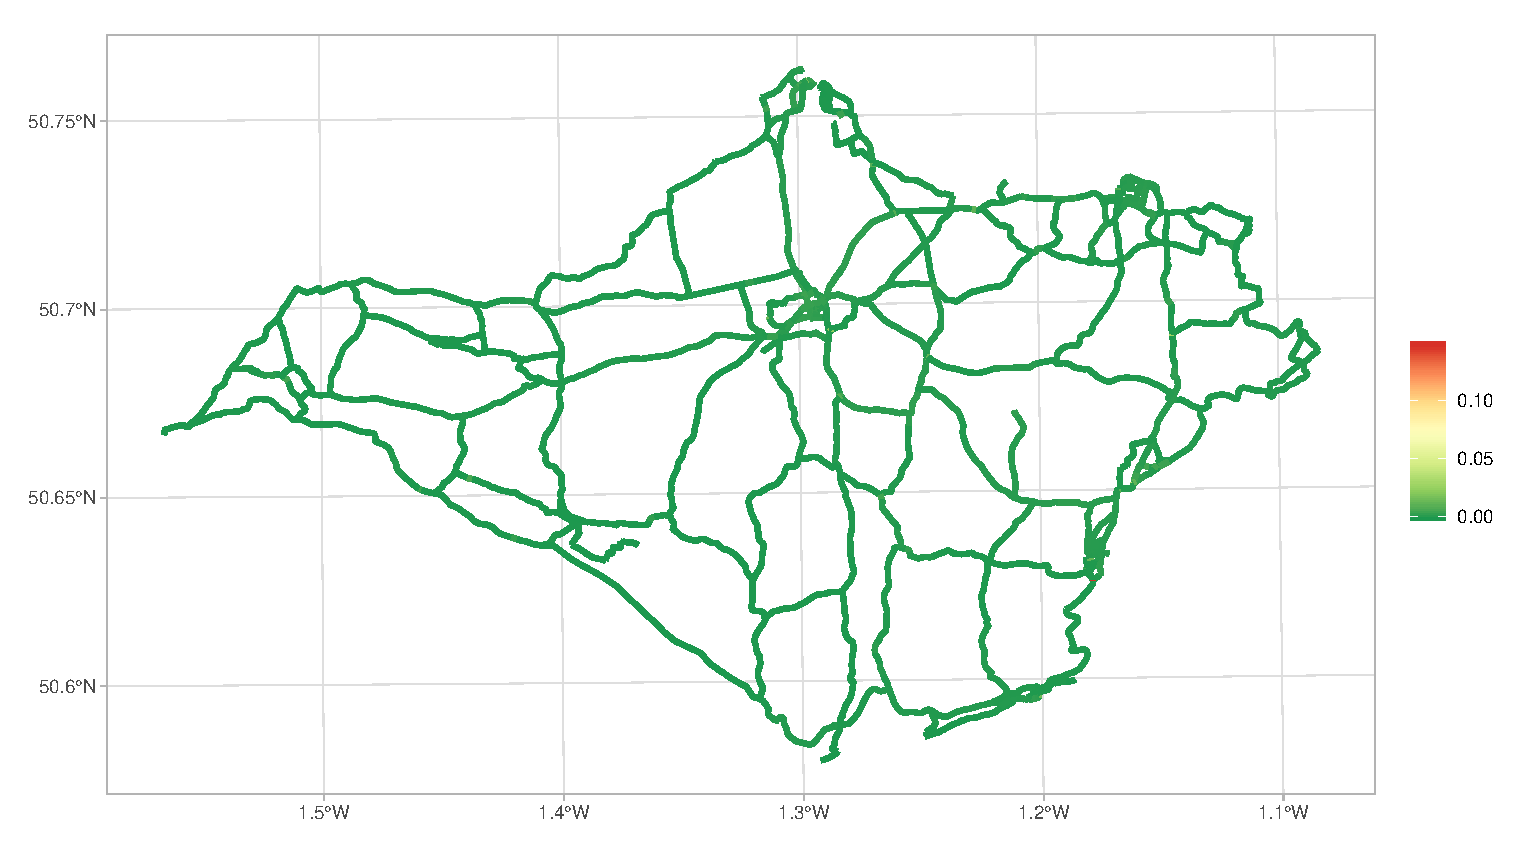
\includegraphics[width=\linewidth]{images/empirical_bayes_1}
\end{figure}
\end{frame}

\begin{frame}
\frametitle{The lengths of the OSM ways data}
\vspace{-0.75cm}
\begin{itemize}
	\setlength\itemsep{1em}
	\item The problem is that $\hat{\theta}_i$ is a convex combination between the number of car crashes per meter and a local average measure where the weights are defined by $P_i = \frac{\sigma^2_i}{\sigma^2_i + \frac{\mu_i}{l_i}}$. 
	
	\item In our case it occurred (by chance) that a few car crashes happened really close to the short edges in the network while all the other surrounding ways remained "empty". This means that $P_i \to 1$, $\hat{\theta}_i \to y_i$ and our methodology fails to solve that problem.
	
	\item  We need an algorithm to \alert{merge the shortest $z\%$ of segments with its nearest and shortest neighbour}. We choose $z = 15\%$. 
\end{itemize}
\end{frame}

\begin{frame}
\frametitle{Merging the shortest segments}
\vspace{-0.5cm}
We \href{https://github.com/ropensci/stplanr/issues/359}{just} started working on this topic, so please don't judge me \dots
\begin{figure}
	\centering
	
\includegraphics[height=0.7\textheight]{images/js.jpeg}\\
	\hspace*{15pt}\hbox{\scriptsize Credit:\thinspace{\small\itshape Subreddit - ProgrammerHumor, User: tetenric}}
\end{figure}
\end{frame}

\begin{frame}[fragile]
\frametitle{Merging the shortest segments}
\vspace{-0.5cm}
This is the pseudo-code:

\begin{algorithm}[H]
	\begin{algorithmic}[1]
		\STATE {Set minimal length threshold.} 
		\STATE {Extract the \texttt{sfc} from the \texttt{sf} object and sort it according to its length}. 
		\STATE Estimate the neighborhood structure. 
		\WHILE{Any segment is longer than threshold}{
			\FOR{$i = 1$ to $length(sfc)$}
			\IF{$st\_length(sfc[i]) > threshold$}
				\STATE Merge the small segment with its nearest and shortest neighbour;
				\STATE Remove the old segments and add the new one;
				\STATE Rebuild the neighborhood structure and sort the \texttt{sfc};
				\STATE BREAK.
			\ENDIF
			\ENDFOR
		}
		\ENDWHILE
	\end{algorithmic}
\end{algorithm}
\end{frame}

\begin{frame}
\vspace{-0.25cm}
\frametitle{The final result}
This is the result with $p = 1$. I think that the methodology is really good but, to be honest, I used a square-root transformation of the empirical bayes estimates just to improve the graphical representation. 
\begin{figure}
	\centering
	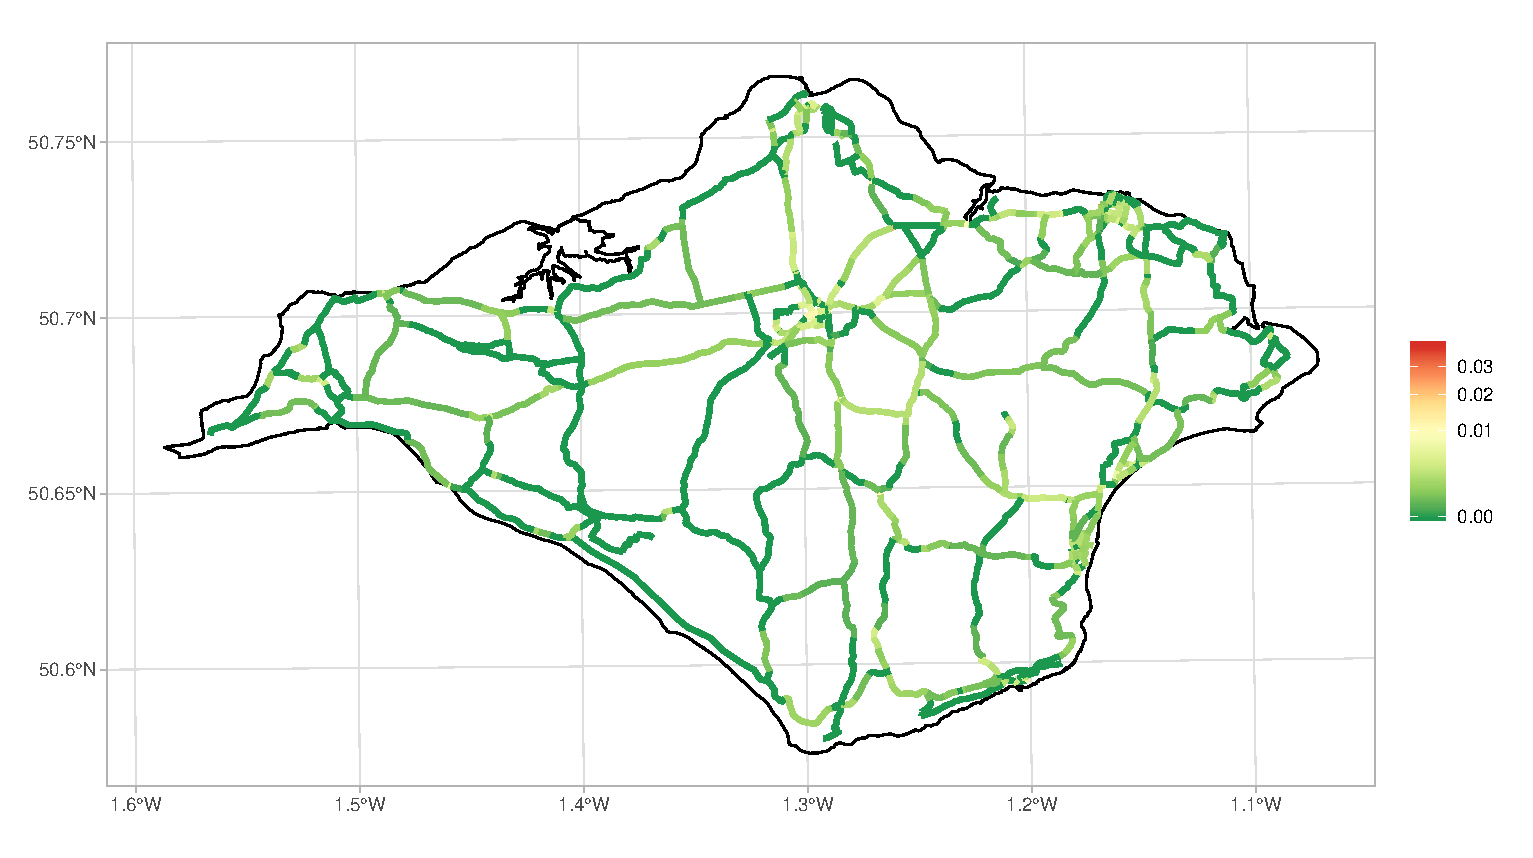
\includegraphics[width=\linewidth]{images/empirical_bayes_2}
\end{figure}
\end{frame}


\begin{frame}[t,allowframebreaks]
\frametitle{Future Works}
\begin{itemize}
	\setlength\itemsep{1em}
	\item Define a proper methodology that takes into account also the severity of car crashes.
	\item Explore several measures of spatial autocorrelation to decide the value of $p$ (like Moran's $I$). 
	\item Properly define $l_i$ as a function of: edge length, Average Annual Daily Traffic, highway type, distance to the nearest intersection and so on\dots (Ideas?).
	\item Take into account the variability associated with the prediction of $l_i$.
	\item Explore the possibility to define a proper prior for $\theta_{i}$. 
	\item Check the differences with more complex and structured spatial bayesian models (i.e. CAR models with MCMC inference).
	 \item Define a proper algorithm for cutting and pasting the edges in the street network. 
\end{itemize}
\end{frame}

\begin{frame}
\frametitle{Final Credits}
\vspace{-0.75cm}
\begin{itemize}
	\setlength\itemsep{1em}
	\item Beamer theme: \href{https://it.overleaf.com/latex/templates/modele-de-presentation-telecom-bretagne/fmthsbxrwcdd}{https://it.overleaf.com/latex/templates/modele-de-presentation-telecom-bretagne/fmthsbxrwcdd}
\end{itemize}
\end{frame}

\begin{frame}[t,allowframebreaks]
\nocite{*}
\frametitle{References}
\printbibliography
\end{frame}

\end{document}



